\section{From motions to a single relaxation}\label{sec:reduction}

We show that a sofa of large area lies in an intersection of hallways as in \cref{def:G}, for suitable angle sets $A$ and $B$, so that its area is at most $G(A;B)$. When we say that a sofa turns right, turns left or passes through $Z_D$, we fix a motion as in \cref{def:sofa} or \cref{def:z} and write $\theta(t)$ and $S_t$ for its orientation and positions. Throughout, $T>\sqrt2$ is a threshold, and we write
\[
\delta_T=\arcsin(1/T), \qquad \gamma_T=\arccos(1/T)=90\dg-\delta_T .
\]
Since $T>\sqrt2$ we have $\delta_T<45\dg<\gamma_T$. \Cref{lem:strips} explains the role of $\delta_T$: a sofa $S\subset H$ of area greater than $T$ can be moved into a vertical strip of width $1$ only when its orientation is within $\delta_T$ of an odd multiple of $90\dg$, and into a horizontal one only when it is within $\delta_T$ of a multiple of $180\dg$.

\needspace{10\baselineskip}
\subsection{Two hallways}\label{sec:twocorridors}

\begin{lem}[No sideways turn]\label{lem:noside}
Let $S$ be a sofa with $\lambda(S)>\sqrt2$, and let $(\theta,\mathbf{x})$ be a motion.
\begin{enumerate}[label=(\roman*)]
\item If the motion moves $S$ around the right turn as in \cref{def:sofa}(c), then $-135\dg<\theta(t)<45\dg$ for all $t$.
\item If the motion moves $S$ around the left turn, then $-45\dg<\theta(t)<135\dg$ for all $t$.
\end{enumerate}
\end{lem}

\begin{proof}
(i) For every $t$ we have $S_t\subset L_0$, so $S\subset L_{-\theta(t)}(\bu)$ for some $\bu$ by \cref{lem:frame}(i); also $S\subset\Lh\subset H$. If $\theta(t)$ were equal to $45\dg$ modulo $180\dg$, the hallway $L_{-\theta(t)}(\bu)$ would be $L_{-45\dg}(\bu)$ or $L_{135\dg}(\bu)$, and \cref{lem:sideways} would give $\lambda(S)\le\sqrt2$. So $\theta$ never takes a value in $45\dg+180\dg\Z$. Since $\theta$ is continuous and $\theta(0)=0$, it stays strictly between the two neighbouring values $-135\dg$ and $45\dg$.

(ii) The same argument with \cref{lem:frame}(ii) excludes the values in $-45\dg+180\dg\Z$.
\end{proof}

\begin{prop}[Turning the right way]\label{prop:natural}
Let $T>\sqrt2$ and let $S$ be a sofa with $\lambda(S)>T$.
\begin{enumerate}[label=(\roman*)]
\item If $S$ turns right, then for every $a\in[0\dg,\gamma_T]$ there is $\bu\in\R^2$ with $S\subset L_a(\bu)$.
\item If $S$ turns left, then for every $b\in[0\dg,\gamma_T]$ there is $\bv\in\R^2$ with $S\subset\rho(L_b(\bv))$.
\end{enumerate}
\end{prop}

\begin{proof}
(i) At the end of the motion $S_1\subset\Lv\subset V$, while $S\subset H$. By \cref{lem:strips}(i), $|\cos\theta(1)|\le1/\lambda(S)<1/T=\sin\delta_T$, so $\theta(1)$ lies within $\delta_T$ of an odd multiple of $90\dg$. By \cref{lem:noside}(i), $\theta(1)$ also lies in $(-135\dg,45\dg)$. Since $\delta_T<45\dg$, the only possibility is $-90\dg-\delta_T<\theta(1)<-90\dg+\delta_T$, and in particular $\theta(1)<-\gamma_T$. As $\theta(0)=0$, the intermediate value theorem gives, for every $a\in[0\dg,\gamma_T]$, a time $t$ with $\theta(t)=-a$, and then $S\subset L_a(\bu)$ for some $\bu$ by \cref{lem:frame}(i).

(ii) In the same way, \cref{lem:strips}(i) and \cref{lem:noside}(ii) give $90\dg-\delta_T<\theta(1)<90\dg+\delta_T$. So $\theta$ takes every value $b\in[0\dg,\gamma_T]$, and \cref{lem:frame}(ii) gives $S\subset\rho(L_b(\bv))$.
\end{proof}

\Cref{lem:noside,prop:natural} are a variant of an argument of Gerver \cite[p.~271]{gerver1992}, in the form given by Baek \cite[Theorem~1.5.1]{baek2024}, who uses it to show that a moving sofa of area at least $2.2$ admits a motion that rotates by at least $\sec^{-1}(2.2)\approx63\dg$. The argument uses only the continuity of the motion and its final position; no monotonicity is assumed. In the ordinary problem, where the areas of interest are about $2.2$, it gives hallways $L_a(\bu)$ only for angles $a$ up to about $63\dg$; the relaxations of \cite{kallusromik2018} also use larger angles, and for these Kallus and Romik rely on Gerver's theorem.

\begin{thm}[Reduction for two hallways]\label{thm:reduction2}
Let $T>\sqrt2$, and let $A,B\subset[0\dg,\gamma_T]$ be finite. Then every ambidextrous sofa $S$ satisfies $\lambda(S)\le\max\{T,\,G(A;B)\}$. Hence $\muA\le\max\{T,G(A;B)\}$.
\end{thm}

\begin{proof}
If $\lambda(S)>T$, then by \cref{prop:natural} $S$ lies in a hallway $L_a(\bu_a)$ for each $a\in A$ and in a mirrored hallway $\rho(L_b(\bv_b))$ for each $b\in B$. Since also $S\subset\Lh\subset H$, \cref{lem:relax} gives $\lambda(S)\le G(A;B)$.
\end{proof}

\subsection{The Z-shaped corridor}\label{sec:zproof}

In the corridor $Z_D$ the sofa first turns left, around the lower corner, and then right, around the upper corner. The two turns happen during a single motion, and a priori the sofa might be in both corners at once, or begin one turn before it has finished the other. We rule this out by showing that a sofa of area greater than $\sqrt2$ is shorter than the vertical section of the corridor. We use two regions of $Z_D$ (\cref{fig:zproof}(a)):
\[
\Lo=Z_D\cap\{y\le D-\tfrac12\}, \qquad \Up=Z_D\cap\{y\ge\tfrac32\}.
\]
For $D\ge2$ they overlap in the rectangle $\Lo\cap\Up=[0,1]\times[\frac32,D-\frac12]$ of the vertical section, and
\begin{equation}\label{eq:LoUp}
\Lo\subset\rho(L_0), \qquad \Up\subset R_{90\dg}L_0+(1,D),
\end{equation}
since $R_{90\dg}L_0+(1,D)=\big([0,1]\times(-\infty,D+1]\big)\cup\big([0,\infty)\times[D,D+1]\big)$.

\begin{figure}[t]
\centering
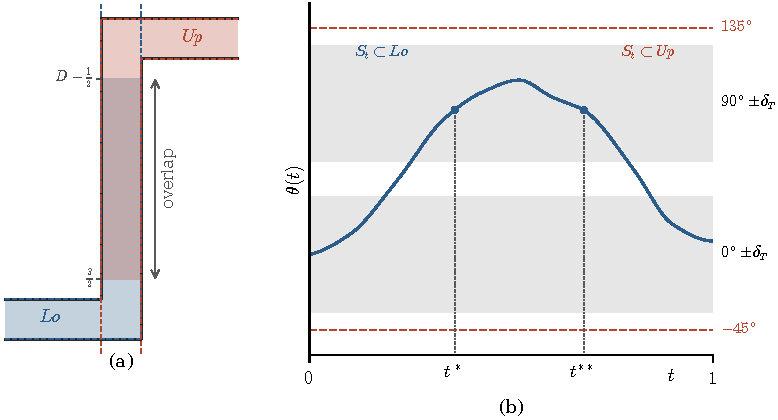
\includegraphics[width=\textwidth]{figures/fig_zproof.pdf}
\caption{(a) The corridor $Z_D$ (here $D=7$) with its lower region $\Lo$ and its upper region $\Up$. The dashed lines show the hallways $\rho(L_0)$ and $R_{90\dg}L_0+(1,D)$ that contain them. (b) A schematic picture of the orientation $\theta(t)$ of a sofa of area greater than $T$ passing through $Z_D$. The orientation never reaches $-45\dg$ or $135\dg$. At the times $t^*$ and $t^{**}$ of \cref{thm:reductionZ} the sofa lies in the overlap of $\Lo$ and $\Up$, so its orientation is within $\delta_T$ of $90\dg$ there; the grey bands have half-width $\delta_T$ for $T=\Tmain$.}
\label{fig:zproof}
\end{figure}

\needspace{10\baselineskip}
\begin{lem}[No sideways position in $Z_D$]\label{lem:zside}
Every line $x+y=c$ meets $Z_D$ in a segment of length $\sqrt2$. Consequently, if a sofa $S$ with $\lambda(S)>\sqrt2$ passes through $Z_D$ with the motion $(\theta,\mathbf{x})$, then $-45\dg<\theta(t)<135\dg$ for all $t$.
\end{lem}

\begin{proof}
A direct check shows that the projection to the $x$-axis of the intersection of $Z_D$ with the line $x+y=c$ is $[c-1,c]$ if $c\le1$, $[0,1]$ if $1\le c\le D+1$, and $[c-D-1,c-D]$ if $c\ge D+1$. In each case the intersection is a segment of length $\sqrt2$.

Now suppose that $\theta(t)$ equals $-45\dg$ modulo $180\dg$ for some $t$. Then $S\subset H\cap R_{-\theta(t)}(Z_D-\mathbf{x}(t))$. The rigid motion $z\mapsto R_{\theta(t)}z+\mathbf{x}(t)$ maps horizontal lines to lines of slope $-1$, so every horizontal line meets $R_{-\theta(t)}(Z_D-\mathbf{x}(t))$ in a segment of length $\sqrt2$, and hence $\lambda(S)\le\sqrt2$, a contradiction. By continuity, $\theta$ stays between $-45\dg$ and $135\dg$.
\end{proof}

\needspace{6\baselineskip}
\begin{lem}[A sofa of area greater than $\sqrt2$ is short]\label{lem:diameter}
Let $D\ge4$. If a sofa $S$ with $\lambda(S)>\sqrt2$ passes through $Z_D$, then $\diam S<5$.
\end{lem}

\begin{proof}
The idea is that the sofa must reach orientation $45\dg$ while it is still in the lower region, and at that moment it lies in a hallway $\rho(L_{45\dg}(\bv))$, which forces it to be short by \cref{lem:width}.

By \cref{lem:bounded}, $S$ is compact. The set of times $t$ with $S_t\subset\Lo$ is closed and contains $0$. Let $\tau$ be the largest time such that $S_t\subset\Lo$ for all $t\in[0,\tau]$. Then $\tau<1$, since $S_1\subset A_2$ is disjoint from $\Lo$. The maximum height $h(t)$ of the points of $S_t$ depends continuously on $t$, because $S$ is compact. Therefore $h(\tau)=D-\frac12$: otherwise $h(t)<D-\frac12$ for all $t$ near $\tau$, and then $S_t\subset Z_D\cap\{y<D-\frac12\}\subset\Lo$ for all $t$ slightly larger than $\tau$.

We claim that $\theta(\tau)\ge45\dg$. Suppose instead that $\theta(\tau)<45\dg$; then $-45\dg<\theta(\tau)<45\dg$ by \cref{lem:zside}. The set $S_\tau$ lies in the strip $R_{\theta(\tau)}H+\mathbf{x}(\tau)$, of width $1$, whose direction makes an angle of less than $45\dg$ with the horizontal. Above the interval $0\le x\le1$, this strip spans a range of heights of length at most $1/\cos\theta(\tau)+|\tan\theta(\tau)|<\sqrt2+1$. Since $S_\tau$ contains a point at height $D-\frac12>1$, and such points of $\Lo$ have $0\le x\le 1$, every point of the strip above $[0,1]$ has height greater than $D-\frac12-(\sqrt2+1)>1$, using $D\ge4$.

Thus the strip avoids the unit square $[0,1]^2$. Now $\Lo$ is the union of $A_1$ and $[0,1]\times[0,D-\frac12]$, and these two sets meet only in $[0,1]^2$. So $S_\tau$ is contained in the union of two disjoint closed sets, one inside $A_1$ and one inside $[0,1]\times[0,D-\frac12]$. Since $S_\tau$ is connected and contains a point of height $D-\frac12$, it lies in the second set, and hence in $V$. Now \cref{lem:strips}(i) gives $\lambda(S)\le1/\cos\theta(\tau)<\sqrt2$, a contradiction.

So $\theta(\tau)\ge45\dg$, and by the intermediate value theorem $\theta(t_0)=45\dg$ for some $t_0\in[0,\tau]$. As $S_{t_0}\subset\Lo\subset\rho(L_0)$, \cref{lem:frame}(ii) gives $S\subset H\cap\rho(L_{45\dg}(\bv))$ for some $\bv$. By \cref{lem:width}, $\diam S\le\sqrt{W_{45\dg}^2+1}=\sqrt{13+8\sqrt2}<5$.
\end{proof}

\begin{lem}[One corner at a time]\label{lem:onecorner}
Let $D\ge7$, and let $S$ be a sofa with $\lambda(S)>\sqrt2$ that passes through $Z_D$. Then at every time $t$, either $S_t\subset\Lo$ or $S_t\subset\Up$.
\end{lem}

\begin{proof}
By \cref{lem:diameter}, $\diam S_t<5\le D-2$. So $S_t$ cannot contain both a point of height less than $\frac32$ and a point of height greater than $D-\frac12$. If $S_t$ has no point above height $D-\frac12$, it lies in $\Lo$. Otherwise it has no point below height $\frac32$, and it lies in $\Up$.
\end{proof}

The constant $7$ is not optimal: moving the thresholds $\frac32$ and $D-\frac12$ closer to $1$ and $D$ gives a slightly smaller value. We have not looked for the smallest $D$ for which the argument works.

\begin{thm}[Reduction for the Z-shaped corridor]\label{thm:reductionZ}
Let $T>\sqrt2$ and $D\ge7$, and let $A\subset[\delta_T,\gamma_T]$ and $B\subset[0\dg,\gamma_T]$ be finite. Then every sofa $S$ that passes through $Z_D$ satisfies $\lambda(S)\le\max\{T,G(A;B)\}$. Hence $\muZ(D)\le\max\{T,G(A;B)\}$.
\end{thm}

\begin{proof}
Suppose $\lambda(S)>T$. Let $\mathcal{T}_{\mathrm{lo}}$ and $\mathcal{T}_{\mathrm{up}}$ be the sets of times $t$ with $S_t\subset\Lo$ and $S_t\subset\Up$ respectively. Both are closed, their union is $[0,1]$ by \cref{lem:onecorner}, and $0\in\mathcal{T}_{\mathrm{lo}}\setminus\mathcal{T}_{\mathrm{up}}$, $1\in\mathcal{T}_{\mathrm{up}}\setminus\mathcal{T}_{\mathrm{lo}}$. Let $t^*$ be the smallest element of $\mathcal{T}_{\mathrm{up}}$ and $t^{**}$ the largest element of $\mathcal{T}_{\mathrm{lo}}$. Every time before $t^*$ lies in $\mathcal{T}_{\mathrm{lo}}$, and this set is closed, so $t^*\in\mathcal{T}_{\mathrm{lo}}$. In the same way $t^{**}\in\mathcal{T}_{\mathrm{up}}$. So at both times the sofa lies in $\Lo\cap\Up\subset V$.

By \cref{lem:strips}(i) and \cref{lem:zside}, $\theta(t^*)$ and $\theta(t^{**})$ lie within $\delta_T$ of $90\dg$. At the end, $S_1\subset A_2$ lies in a horizontal strip, so by \cref{lem:strips}(ii) and \cref{lem:zside}, $\theta(1)$ lies within $\delta_T$ of $0\dg$.

\emph{The left turn.} For $t\in[0,t^*]$ we have $S_t\subset\Lo\subset\rho(L_0)$ by \eqref{eq:LoUp}, so $S\subset\rho(L_{\theta(t)}(\bv))$ for some $\bv$ by \cref{lem:frame}(ii). Since $\theta(0)=0$ and $\theta(t^*)>90\dg-\delta_T=\gamma_T$, every $b\in[0\dg,\gamma_T]$ is a value of $\theta$ on $[0,t^*]$. So $S$ lies in a mirrored hallway $\rho(L_b(\bv_b))$ for every $b\in B$.

\emph{The right turn.} For $t\in[t^{**},1]$ we have $S_t\subset\Up\subset R_{90\dg}L_0+(1,D)$, so $S\subset L_{90\dg-\theta(t)}(\bu)$ for some $\bu$ by \cref{lem:frame}(iii). Since $\theta(t^{**})>90\dg-\delta_T$ and $\theta(1)<\delta_T$, the angle $90\dg-\theta(t)$ takes every value in $[\delta_T,\gamma_T]$ on $[t^{**},1]$. So $S$ lies in a hallway $L_a(\bu_a)$ for every $a\in A$.

Finally $S\subset A_1\subset H$, and \cref{lem:relax} gives $\lambda(S)\le G(A;B)$.
\end{proof}

The condition $A\subset[\delta_T,\gamma_T]$, rather than $A\subset[0\dg,\gamma_T]$, is needed because the right turn does not start from a known orientation: at the time $t^{**}$ we only know that $|90\dg-\theta(t^{**})|<\delta_T$, so angles in $[0\dg,\delta_T)$ need not be visited during the right turn. The upper limit $\gamma_T$ comes from the final orientation, as in \cref{thm:reduction2}.

\subsection{Proof of \texorpdfstring{\cref{thm:hand}}{Theorem 1.2}}\label{sec:proofhand}

Let $T=2\sqrt2-1>\sqrt2$, so that $\delta_T<45\dg<\gamma_T$. Taking $A=B=\{45\dg\}$ in \cref{thm:reduction2,thm:reductionZ}, and using $G(\{45\dg\};\{45\dg\})=2\sqrt2-1$ from \cref{prop:onehalf}, we obtain $\lambda(S)\le 2\sqrt2-1$ for every ambidextrous sofa and for every sofa that passes through $Z_D$ with $D\ge7$. \qed
